%-----------------------------------------------------------------------------------------------------------------------------------------------%
%	The MIT License (MIT)
%
%	Copyright (c) 2019 Jan Küster
%
%	Permission is hereby granted, free of charge, to any person obtaining a copy
%	of this software and associated documentation files (the "Software"), to deal
%	in the Software without restriction, including without limitation the rights
%	to use, copy, modify, merge, publish, distribute, sublicense, and/or sell
%	copies of the Software, and to permit persons to whom the Software is
%	furnished to do so, subject to the following conditions:
%
%	THE SOFTWARE IS PROVIDED "AS IS", WITHOUT WARRANTY OF ANY KIND, EXPRESS OR
%	IMPLIED, INCLUDING BUT NOT LIMITED TO THE WARRANTIES OF MERCHANTABILITY,
%	FITNESS FOR A PARTICULAR PURPOSE AND NONINFRINGEMENT. IN NO EVENT SHALL THE
%	AUTHORS OR COPYRIGHT HOLDERS BE LIABLE FOR ANY CLAIM, DAMAGES OR OTHER
%	LIABILITY, WHETHER IN AN ACTION OF CONTRACT, TORT OR OTHERWISE, ARISING FROM,
%	OUT OF OR IN CONNECTION WITH THE SOFTWARE OR THE USE OR OTHER DEALINGS IN
%	THE SOFTWARE.
%
%
%-----------------------------------------------------------------------------------------------------------------------------------------------%


%============================================================================%
%
%	DOCUMENT DEFINITION
%
%============================================================================%

%we use article class because we want to fully customize the page and don't use a cv template
\documentclass[10pt,A4]{article}


%----------------------------------------------------------------------------------------
%	ENCODING
%----------------------------------------------------------------------------------------

% we use utf8 since we want to build from any machine
\usepackage[utf8]{inputenc}

%----------------------------------------------------------------------------------------
%	LOGIC
%----------------------------------------------------------------------------------------

% provides \isempty test
\usepackage{xstring, xifthen}

\usepackage{enumitem}

%----------------------------------------------------------------------------------------
%	FONT BASICS
%----------------------------------------------------------------------------------------

% some tex-live fonts - choose your own

%\usepackage[defaultsans]{droidsans}
%\usepackage[default]{comfortaa}
%\usepackage{cmbright}
\usepackage[default]{raleway}
%\usepackage{fetamont}
%\usepackage[default]{gillius}
%\usepackage[light,math]{iwona}
%\usepackage[thin]{roboto}

% set font default
\renewcommand*\familydefault{\sfdefault}
\usepackage[T1]{fontenc}

% more font size definitions
\usepackage{moresize}

%----------------------------------------------------------------------------------------
%	FONT AWESOME ICONS
%----------------------------------------------------------------------------------------

% include the fontawesome icon set
\usepackage{fontawesome}

% use to vertically center content
% credits to: http://tex.stackexchange.com/questions/7219/how-to-vertically-center-two-images-next-to-each-other
\newcommand{\vcenteredinclude}[1]{\begingroup
\setbox0=\hbox{\includegraphics{#1}}%
\parbox{\wd0}{\box0}\endgroup}

% use to vertically center content
% credits to: http://tex.stackexchange.com/questions/7219/how-to-vertically-center-two-images-next-to-each-other
\newcommand*{\vcenteredhbox}[1]{\begingroup
\setbox0=\hbox{#1}\parbox{\wd0}{\box0}\endgroup}

% icon shortcut
\newcommand{\icon}[3] {
    \makebox(#2, #2){\textcolor{maincol}{\csname fa#1\endcsname}}
}

% icon with text shortcut
\newcommand{\icontext}[4]{
    \vcenteredhbox{\icon{#1}{#2}{#3}}  \hspace{2pt}  \parbox{0.9\mpwidth}{\textcolor{#4}{#3}}
}

% icon with website url
\newcommand{\iconhref}[5]{
    \vcenteredhbox{\icon{#1}{#2}{#5}}  \hspace{2pt} \href{#4}{\textcolor{#5}{#3}}
}

% icon with email link
\newcommand{\iconemail}[5]{
    \vcenteredhbox{\icon{#1}{#2}{#5}}  \hspace{2pt} \href{mailto:#4}{\textcolor{#5}{#3}}
}

%----------------------------------------------------------------------------------------
%	PAGE LAYOUT  DEFINITIONS
%----------------------------------------------------------------------------------------

% page outer frames (debug-only)
% \usepackage{showframe}

% we use paracol to display breakable two columns
\usepackage{paracol}

% define page styles using geometry
\usepackage[a4paper]{geometry}

% remove all possible margins
\geometry{top=1cm, bottom=1cm, left=1cm, right=1cm}

\usepackage{fancyhdr}
\pagestyle{empty}

% space between header and content
% \setlength{\headheight}{0pt}

% indentation is zero
\setlength{\parindent}{0mm}

%----------------------------------------------------------------------------------------
%	TABLE /ARRAY DEFINITIONS
%----------------------------------------------------------------------------------------

% extended aligning of tabular cells
\usepackage{array}

% custom column right-align with fixed width
% use like p{size} but via x{size}
\newcolumntype{x}[1]{%
        >{\raggedleft\hspace{0pt}}p{#1}}%


%----------------------------------------------------------------------------------------
%	GRAPHICS DEFINITIONS
%----------------------------------------------------------------------------------------

%for header image
\usepackage{graphicx}

% use this for floating figures
% \usepackage{wrapfig}
% \usepackage{float}
% \floatstyle{boxed}
% \restylefloat{figure}

%for drawing graphics
\usepackage{tikz}
\usetikzlibrary{shapes, backgrounds,mindmap, trees}

%----------------------------------------------------------------------------------------
%	Color DEFINITIONS
%----------------------------------------------------------------------------------------
\usepackage{transparent}
\usepackage{color}

% primary color
\definecolor{maincol}{RGB}{ 24, 63, 194 }

% accent color, secondary
% \definecolor{accentcol}{RGB}{ 250, 150, 10 }

% dark color
\definecolor{darkcol}{RGB}{ 70, 70, 70 }

% light color
\definecolor{lightcol}{RGB}{ 200, 200, 200 }


% Package for links, must be the last package used
\usepackage[hidelinks]{hyperref}

% returns minipage width minus two times \fboxsep
% to keep padding included in width calculations
% can also be used for other boxes / environments
\newcommand{\mpwidth}{\linewidth-\fboxsep-\fboxsep}


%============================================================================%
%
%	CV COMMANDS
%
%============================================================================%

%----------------------------------------------------------------------------------------
%	 CV LIST
%----------------------------------------------------------------------------------------

% renders a standard latex list but abstracts away the environment definition (begin/end)
\newcommand{\cvlist}[1] {
    \begin{itemize}[itemsep=3pt,topsep=10pt]{#1}\end{itemize}
}

%----------------------------------------------------------------------------------------
%	 CV TEXT
%----------------------------------------------------------------------------------------

% base class to wrap any text based stuff here. Renders like a paragraph.
% Allows complex commands to be passed, too.
% param 1: *any
\newcommand{\cvtext}[1] {
    \begin{tabular*}{1\mpwidth}{p{0.98\mpwidth}}
        \parbox{1\mpwidth}{#1}
    \end{tabular*}
}

%----------------------------------------------------------------------------------------
%	CV SECTION
%----------------------------------------------------------------------------------------

% Renders a a CV section headline with a nice underline in main color.
% param 1: section title
\newcommand{\cvsection}[1] {
    \vspace{14pt}
    \cvtext{
        \textbf{\LARGE{\textcolor{darkcol}{\uppercase{#1}}}}\\[-4pt]
        \textcolor{maincol}{ \rule{0.1\textwidth}{2pt} } \\
    }
}

%----------------------------------------------------------------------------------------
%	META SKILL
%----------------------------------------------------------------------------------------

% Renders a progress-bar to indicate a certain skill in percent.
% param 1: name of the skill / tech / etc.
% param 2: level (for example in years)
% param 3: percent, values range from 0 to 1
\newcommand{\cvskill}[3] {
    \begin{tabular*}{1\mpwidth}{p{0.72\mpwidth}  r}
        \textcolor{black}{\textbf{#1}} & \textcolor{maincol}{#2}\\
    \end{tabular*}%

    \hspace{4pt}
    \begin{tikzpicture}[scale=1,rounded corners=2pt,very thin]
        \fill [lightcol] (0,0) rectangle (1\mpwidth, 0.15);
        \fill [maincol] (0,0) rectangle (#3\mpwidth, 0.15);
    \end{tikzpicture}%
    \vspace{0pt}
}


%----------------------------------------------------------------------------------------
%	 CV EVENT
%----------------------------------------------------------------------------------------

% Renders a table and a paragraph (cvtext) wrapped in a parbox (to ensure minimum content
% is glued together when a pagebreak appears).
% Additional Information can be passed in text or list form (or other environments).
% the work you did
% param 1: time-frame i.e. Sep 14 - Jan 15 etc.
% param 2:	 event name (job position etc.)
% param 3: Customer, Employer, Industry
% param 4: Short description
% param 5: work done (optional)
% param 6: technologies include (optional)
% param 7: achievements (optional)
\newcommand{\cvevent}[7] {

% we wrap this part in a parbox, so title and description are not separated on a pagebreak
% if you need more control on page breaks, remove the parbox
    \parbox{\mpwidth}{
        \begin{tabular*}{1\mpwidth}{p{0.72\mpwidth}  r}
            \textcolor{black}{\textbf{#2}}   & \colorbox{maincol}{\makebox[0.33\mpwidth]{\textcolor{white}{#1}}} \\
            \textcolor{maincol}{\textbf{#3}} &                                                                   \\
        \end{tabular*}\\[8pt]

        \ifthenelse{\isempty{#4}}{}{
            \cvtext{#4}\\
        }
    }

    \ifthenelse{\isempty{#5}}{}{
        \vspace{9pt}
        {#5}
    }

    \ifthenelse{\isempty{#6}}{}{
        \vspace{9pt}
        \cvtext{\textbf{Technologies include:}}
        {#6}
    }

    \ifthenelse{\isempty{#7}}{}{
        \vspace{9pt}
        \cvtext{\textbf{Achievements include:}}
        {#7}
    }
    \vspace{14pt}
}

%----------------------------------------------------------------------------------------
%	 CV META EVENT
%----------------------------------------------------------------------------------------

% Renders a CV event on the sidebar
% param 1: title
% param 2: subtitle (optional)
% param 3: customer, employer, etc,. (optional)
% param 4: info text (optional)
\newcommand{\cvmetaevent}[4] {
    \textcolor{maincol} {\cvtext{\textbf{\begin{flushleft}
                                             #1
    \end{flushleft}}}}

    \ifthenelse{\isempty{#2}}{}{
        \textcolor{darkcol} {\cvtext{\textbf{#2}} }
    }

    \ifthenelse{\isempty{#3}}{}{
        \cvtext{{ \textcolor{darkcol} {#3} }}\\
    }

    \cvtext{#4}\\[14pt]
}

%---------------------------------------------------------------------------------------
%	QR CODE
%----------------------------------------------------------------------------------------

% Renders a qrcode image (centered, relative to the parentwidth)
% param 1: percent width, from 0 to 1
\newcommand{\cvqrcode}[1] {
    \begin{center}
        \includegraphics[width={#1}\mpwidth]{qrcode}
    \end{center}
}


%============================================================================%
%
%
%
%	DOCUMENT CONTENT
%
%
%
%============================================================================%
\begin{document}
    \columnratio{0.31}
    \setlength{\columnsep}{2.2em}
    \setlength{\columnseprule}{4pt}
    \colseprulecolor{lightcol}
    \begin{paracol}{2}
        \begin{leftcolumn}
%---------------------------------------------------------------------------------------
%	META IMAGE
%----------------------------------------------------------------------------------------
            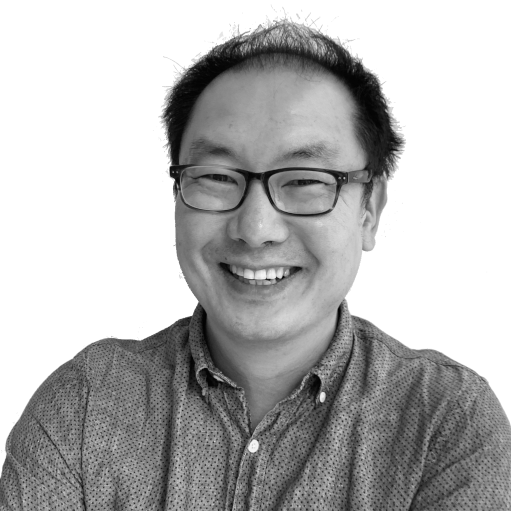
\includegraphics[width=\linewidth]{thomas_han.png}    %trimming relative to image size

%---------------------------------------------------------------------------------------
%	META SKILLS
%----------------------------------------------------------------------------------------
            \cvsection{SKILLS}

            \cvskill{Java} {20+ yrs} {1} \\[-2pt]
            \cvskill{Python} {10+ yrs} {0.9} \\[-2pt]
            \cvskill{HTML/CSS/Javascript} {15+ yrs} {0.75} \\[-2pt]
            \cvskill{SQL} {20+ yrs} {1} \\[-2pt]
            \cvskill{Linux/Windows} {20+ yrs} {1} \\[-2pt]
            \cvskill{Unix} {10+ yrs} {1} \\[-2pt]
            \cvskill{Agile/TDD} {20+ yrs} {1} \\[-2pt]
            \cvskill{Reactive Programming} {8+ yrs} {1} \\[-2pt]
            \cvskill{DevOps} {10+ yrs} {0.8} \\[-2pt]
            \cvskill{Git} {15+ yrs} {1} \\[-2pt]



            \vfill\null
            \cvsection{CONTACT}

            \icontext{MobilePhone}{12}{+61 422 576 435}{black}\\[6pt]
            \iconhref{Globe}{12}{https://hanz.au}{https://hanz.au}{black}\\[6pt]
            \iconhref{LinkedinSquare}{12}{https://www.linkedin.com/\\in/thomas-hanz/}{https://www.linkedin.com/in/thomas-hanz/}{black}\\[6pt]
            \iconemail{Envelope}{12}{thomas.han@live.com}{thomas.han@live.com}{black}\\[6pt]

            \vfill\null
            \cvqrcode{0.7}

%---------------------------------------------------------------------------------------
%	EDUCATION
%----------------------------------------------------------------------------------------
            \newpage
            \cvsection{EDUCATION}

            \cvmetaevent
            {2000 - 2003}
            {BE Electrical Engineering}
            {University of Canterbury}

            \cvmetaevent
            {2004 - 2005}
            {BSc Computer Science}
            {University of Canterbury}

            \cvmetaevent
            {2006 - 2006}
            {MSc Computer Science}
            {University of Canterbury}
            {Not completed}

            \vfill\null
            \cvqrcode{0.7}

%%---------------------------------------------------------------------------------------
%%	CERTIFICATION
%%----------------------------------------------------------------------------------------
%\newpage
%\cvsection{CERTIFICATIONS}
%
%\cvmetaevent
%{LPIC 1 - Linux administrator}
%{}
%{}
%{Certificate issued by the Linux Professional Institute to prove abilities in Linux administration}
%
%\cvmetaevent
%{IBM InfoSphere Advanced DataStage Essentials}
%{}
%{}
%{Intense course about the ETL technologies and the use of IBM DataStage.}
%
%\cvmetaevent
%{Jump Start Program}
%{}
%{}
%{Two months full-time training in object oriented programming in Java SE/EE, software development, testing and modern enterprise web-frameworks. Other topics were object oriented design patterns, test-driven development, SQL-databases and webservers in Java environment (Tomcat / Glasfish / JBoss / Jety)}
%
%
%\cvmetaevent
%{Online Classes}
%{}
%{}
%{It is important for me to stay up to date with the newest topics in the field of IT. In DevOps it is also important to have a general overview and a hands-on experience on them. Therefore, besides intense article studies, I also keep myself up to date with online classes.}
%
%\vfill
%\cvqrcode{0.7}
%
%\newpage
%\mbox{} % hotfix to place qrcode on the bottom when there are not other elements
%\vfill
%\cvqrcode{0.7}

        \end{leftcolumn}
        \begin{rightcolumn}
%---------------------------------------------------------------------------------------
%	TITLE  HEADER
%----------------------------------------------------------------------------------------
            \fcolorbox{white}{darkcol}{\begin{minipage}[c][3.5cm][c]{1\mpwidth}
                                           \begin {center}
                                               \HUGE{ \textbf{ \textcolor{white}{ \uppercase{ Thomas Han } } } } \\[-24pt]
                                               \textcolor{white}{ \rule{0.1\textwidth}{1.25pt} } \\[4pt]
                                               \large{ \textcolor{white} {Head of Engineering} }
                                           \end {center}
            \end{minipage}} \\[14pt]
            \vspace{-12pt}

%---------------------------------------------------------------------------------------
%	PROFILE
%----------------------------------------------------------------------------------------
            \vfill\null
            \cvsection{PROFILE}

            \cvtext{Thomas Han is a Head of Engineering with a focus on creating performant, resilient, scalable software solutions, demonstrating significant expertise in full-stack development.\\

            His leadership at Adnuntius led to notable improvements in system performance and efficiency, especially in high-throughput, low-latency environments.\\

            Thomas has applied his skills across diverse sectors, optimising system functionalities while ensuring data security.\\

            Committed to innovation and the open-source community, he blends technical knowledge with strategic insight, fostering team environments that encourage creativity.}

%---------------------------------------------------------------------------------------
%	WORK EXPERIENCE
%----------------------------------------------------------------------------------------
            \vfill\null
            \cvsection{WORK EXPERIENCE}

            \cvevent
            {Dec 2020 - NOW}
            {Head of Engineering @ Adnuntius}
            {High-throughput, low-latency AdTech}
            {Adnuntius is an AdTech SaaS company that offers products such as Self-Service, Marketplace, Ad Server, and Data to publishers and ad buyers.
            Founded in 2016, Adnuntius enables better control, insight, and flexibility for its customers, as well as next generation advertising without relying on third party data.
            Adnuntius is headquartered in Oslo, Norway with the R\&D centre based in Melbourne.
            The ad server handles over 12 billion requests per month, with high availability and low latency}
            {\cvlist{
                \item Full-stack development across the Adnuntius products (Ad Server, Data analysis, AI, SRE, Performance, DevOps)
                \item Architecting and implementing new features and optimising existing ones
                \item Maintenance/improvement of existing infrastructure
                \item Emergency response and incident management
                \item Strategic planning for future technologies and development
                \item Setup frameworks to measure performance using Gatling and JMH
            }}
            {\cvlist {
                \item Java 17 for majority of the backend
                \item AngularJS for the frontend
                \item Kafka and reactive microservices for high-throughput and low-latency backend
                \item Ansible/bash + Gitlab for 1-click deployments
                \item Docker local developments and CI/CD
                \item Python for system tests
                \item Hybrid AWS/Hetzner for cloud infrastructure
                \item Kubernetes for container orchestration
                \item Hugging face for AI models
            }}
            {\cvlist{
                \item Improved SQL queries by as much as 95\% by careful SQL query planning and denormalisation
                \item Improved throughput by 50\% by utilising concurrency much as possible in the critical areas
                \item Improved ad matching by utilising semantic page matching and AI models
                \item Improved system reliability by implementing monitoring and alerting systems in all mission critical areas
                \item Achieved true CD with multiple deployments per day and automated rollbacks
            }}

            \vfill\null
            \cvevent
            {Sep 2019 - Nov 2020}
            {eFX Engineer @ ANZ}
            {Ultra-low latency trading platform}
            {Responsible for architecting and implementing event based trading platform while ensuring ultra-low latency and high-throughput was achieved.
            Managed the CI/CD process across multiple teams in the eFX domain.}
            {\cvlist{
                \item Extend existing pricing and trading systems to support new events
                \item Develop and profile garbage-free trading systems in Java
                \item Maintain and improve existing CI/CD pipeline
            }}
            {\cvlist {
                \item Java 8
                \item Ultra Messaging
                \item KDB
                \item Chronicle
                \item Ansible
                \item Docker
            }}
            {\cvlist{
                \item Uplifted the DevOps capability across multiple teams using Docker and Ansible
                \item Migrated the entire QA environment into AWS
                \item Improved weekly production deployment process which was unrealiable due to manual deployment
            }}

            \vfill\null
            \cvevent
            {Sep 2018 - Sep 2019}
            {Senior Solution Designer @ nabtrade}
            {Financial trading platform}
            {Responsible for designing the integration of Cash Manager Account (CMA) in nabtrade with various third-party vendors such as FNZ, IRESS and SecuritEase.
            As the lead solution designer, I worked closely with a team of BAs to work out the business requirements and come up with fully functioning software designs for the business requirements.}
            {\cvlist{
                \item Design and document the integration of nabtrade with third-party vendors, and between the third-party vendors
                \item Lead a team of BAs to flush out the requirements
                \item Make POC for the integration
            }}
            {\cvlist {
                \item Spring boot
                \item Kafka
                \item SOAP
                \item IRESS, FNZ and SecuritEase
            }}
            {\cvlist{
                \item Completed the design for locking funds in the CMA account and integrated with the third-party vendor
            }}

            \vfill\null
            \cvevent
            {Jun 2017 - Sep 2018}
            {Distributed Systems Architect / Quant Trader}
            {Financial trading system}
            {Responsible for architecting and building reactive AI trading system.}
            {\cvlist{
                \item Building the AI trading system
                \item Ingest and processs huge datasets with Akka and Spark
                \item Analyse huge datasets with python, Zeppelin
                \item Build AI models with TensorFlow, H2O, Keras
            }}
            {\cvlist {
                \item Multiple JVM languages (Java, Scala, Groovy)
                \item Python and data processing, analysis tools, and AI (Jupyter, Pandas, Numpy, Matplotlib, Dask, Spark, TensorFlow, Keras)
                \item Git
            }}
            {}

            \vfill\null
            \cvevent
            {Mar 2014 - Jun 2017}
            {Lead Full Stack Software Engineer @ Odecee}
            {IT Consultant}
            {Responsible delivering projects across various clients and sectors. My responsibility varied depending on the clients' needs.}
            {\cvlist{
                \item Big Data Architect / Engineer @ Telstra Location Insights Project (Oct 2016 - Jun 2017)
                \item Lead Software Engineer @ NAB E301 Service Engine Project (Dec 2015 - Oct 2016)
                \item Lead Software Engineer @ NAB Accounting Package Integration Project (Nov 2014 - Dec 2015)
                \item Senior Software Engineer @ NAB NextGen Project (Jul 2014 – Nov 2014)
                \item Senior Software Engineer @ Australia Post Enterprise Cloud Platform (ECP) Migration Project (Mar 2014 – Jul 2014)
            }}
            {}
            {}

            \vfill\null
            \cvevent
            {Oct 2016 - Jun 2017}
            {Big Data Architect / Engineer @ Telstra}
            {Insights Project - Big Data Platform}
            {Responsible for implementing algorithms in Spark to uncover insights into people movements in the telco network.}
            {\cvlist{
                \item Implementing algorithms in Spark and uncovering insights using data analysis tools in Zeppelin
                \item Architecting and building the data pipeline for efficient data processing of huge datasets
                \item Architecting and building the data privacy and security frameworks for data protection, both for in transit and at rest data
                \item Building streaming data pipelines for real-time data processing using Nifi and Spark Streaming
            }}
            {\cvlist {
                \item Scala
                \item Spark
                \item Hadoop
                \item Hive
                \item YARN
                \item Kafka, Zookeeper
                \item Nifi
            }}
            {}

            \vfill\null
            \cvevent
            {Dec 2015 - Oct 2016}
            {Lead Software Engineer @ NAB}
            {E301 Service Engine - Banking API}
            {Responsible for leading a squad which implemented API to expose core banking functionalities to internal and external systems. The API eventually morphed into Open Banking API.}
            {\cvlist{
                \item Implementing microservice and exposing the API using Spring Boot
                \item Measure and improve performance of the API using Gatling and JMeter
            }}
            {\cvlist {
                \item Java 8
                \item Spring Boot
                \item JHadoop
                \item Hive
                \item YARN
                \item Kafka, Zookeeper
                \item Nifi
            }}
            {}

            \vfill\null
            \cvevent
            {Nov 2014 - Dec 2015}
            {Lead Software Engineer @ NAB}
            {Accounting Package Integration Project - Loan Services API}
            {Responsible for full SDLC of the loan services API from inception to post-support.
            The API was integrated with major accounting systems like Xero and Quickbooks so automated decisions on QuickBiz loans could be made.}
            {\cvlist{
                \item Implementing API using Play
            }}
            {\cvlist {
                \item Java 8
                \item Play
                \item SQL
            }}
            {}

            \vfill\null
            \cvevent
            {Jul 2014 – Nov 2014}
            {Senior Software Engineer @ NAB}
            {NextGen MyTracker App - SPA Using AngularJS}
            {Responsible for building the SPA MyTracker App in AngularJS. The SPA was used by the NAB's personal banking customers streamline processing credit card applications.}
            {\cvlist{
                \item Implementing SPA using AngularJS
            }}
            {\cvlist {
                \item AngularJS
                \item Node.js
            }}
            {}

            \vfill\null
            \cvevent
            {Mar 2014 – Jul 2014}
            {Senior Software Engineer @ Australia Post}
            {Enterprise Cloud Platform (ECP) Migration}
            {Responsible migrating Australia Post's internal applications from Hostworks into AWS.}
            {\cvlist{
                \item Migrating existing applications into AWS
                \item Making the new applications cloud-ready
            }}
            {\cvlist {
                \item AWS
                \item Spring Boot
            }}
            {}

            \vfill\null
            \cvevent
            {Nov 2013 – Mar 2014}
            {Java Developer @ SecurePay}
            {Post Billpay Migration}
            {Responsible migrating Australia Post's payment system to SecurePay's infrastructure.
            This included all online payments, IVR and operator-assisted payments.}
            {}
            {\cvlist {
                \item Java, Groovy
                \item Spring Boot
            }}
            {}

            \vfill\null
            \cvevent
            {Oct 2012 – Sep 2013}
            {Team Lead @ Australia Post}
            {FlexiPOS EFT Banking}
            {Responsible building FlexiPOS which is an existing POS solution for low volume outlets which allow bill payments, article scanning, and postage assessments. \\
            The lack of card payment meant outlets were only allowed to accept cash or cheque as the only valid form of payment. \\
            This project enabled card payments and banking functions such as deposits to be done by relying on cloud computing solution from Quest.}
            {}
            {\cvlist {
                \item Groovy, Grails
                \item Spring Security
                \item Selenium
                \item JMS
                \item jQuery
                \item Quartz
                \item WebLogic
                \item SVN
            }}
            {}

            \vfill\null
            \cvevent
            {Oct 2012 – Sep 2013}
            {Team Lead @ Australia Post}
            {FlexiPOS EFT Banking and My Deliveries}
            {Responsible building FlexiPOS which is an existing POS solution for low volume outlets which allow bill payments, article scanning, and postage assessments. \\
            The lack of card payment meant outlets were only allowed to accept cash or cheque as the only valid form of payment. \\
            This project enabled card payments and banking functions such as deposits to be done by relying on cloud computing solution from Quest.}
            {}
            {\cvlist {
                \item Groovy, Grails
                \item Spring Security
                \item Selenium
                \item JMS
                \item jQuery
                \item Quartz
                \item WebLogic
                \item SVN
            }}
            {}

            \vfill\null
            \cvevent
            {October 2011 – October 2012}
            {Senior Software Engineer/Consultant @ DiUS}
            {IT Consultant}
            {Responsible for building and delivering projects across various clients}
            {\cvlist{
                \item Senior Software Engineer @ Australia Post Digital Mailbox
                \item Senior Software Engineer @ Percepscion PowerVu
                \item Senior Software Engineer @ Jemena AMI
                \item Senior Software Engineer @ Taylor Ventures
                \item Senior Software Engineer @ Open Universities Australia (OUA) Career Advisor
            }}
            {}
            {}

            \vfill\null
            \cvevent
            {Nov 2008 – Jul 2011}
            {Software Engineer @ Alchemy Group Limited}
            {IT Consultant}
            {Responsible for building applications for various clients}
            {\cvlist{
                \item Assembly School Management System (www.assembly-sms.co.nz)
                \item NZSki (www.nzski.com)
                \item Payment gateway for NZSki MyPass (www.nzski.com/mypass)
            }}
            {}
            {}

            \vfill\null
            \cvevent
            {Apr 2008 – Nov 2008}
            {Web developer @ artworks.net.nz}
            {Web development}
            {Responsible for building and maintaining the over 200 websites and eCommerce solutions for the artworks.net.nz clients.}
            {}
            {}
            {}

            \vfill\null
            \cvevent
            {Dec 2005 – Apr 2008}
            {Software Developer @ Clickserv}
            {Web development and eCommerce}
            {Responsible for building and maintaining eCommerce solutions.}
            {}
            {}
            {}

% hotfixes to create fake-space to ensure the whole height is used
            \mbox{}
            \vfill
            \mbox{}
            \vfill
            \mbox{}
            \vfill
            \mbox{}
        \end{rightcolumn}
    \end{paracol}
\end{document}
